
%(BEGIN_QUESTION)
% Copyright 2006, Tony R. Kuphaldt, released under the Creative Commons Attribution License (v 1.0)
% This means you may do almost anything with this work of mine, so long as you give me proper credit

A vessel holding some process liquid needs to have its level monitored.  The range of level in this vessel is 0 to 20 feet, and the process liquid has a specific gravity of 1.0 (like water).  Someone decides to attach a pressure transmitter to the bottom of the vessel to infer level from hydrostatic pressure like this:

$$\includegraphics[width=15.5cm]{i00248x01.eps}$$

Later, a top is added to this vessel to keep rain from entering in.  Unfortunately, though, this process liquid tends to emit vapor which will be trapped by the closed vessel and create a pressure inside of it.  A small vent is added to the top of the vessel to permit the vapor to escape, but it is a {\it small} vent, not big enough to ensure a total absence of vapor pressure buildup at all times:

$$\includegraphics[width=15.5cm]{i00248x02.eps}$$

What problem in level measurement will result from there being an occasional vapor pressure buildup inside this vessel?  How may this problem be corrected so that the liquid level will be accurately measured at all times?

\underbar{file i00248}
%(END_QUESTION)





%(BEGIN_ANSWER)

Any vapor pressure will be sensed by the transmitter and interpreted as increased liquid level!

\vskip 10pt

Two solutions to this problem: 

\vskip 10pt {\narrower \noindent \baselineskip5pt

(1) Use two transmitters (one at top of vessel, one at bottom) and electronically subtract their output signals.

\par} \vskip 10pt



\vskip 10pt {\narrower \noindent \baselineskip5pt

(2) Connect the ``Low'' side of the one $\Delta$P transmitter to the top of the vessel to naturally compensate for vapor pressure.

\par} \vskip 10pt

Since the transmitter infers level from the amount of pressure sensed at the bottom of the vessel, any vapor pressure buildup inside the vessel will be falsely interpreted as additional liquid level, since the transmitter senses the {\it sum total} of hydrostatic pressure plus any vapor pressure trapped inside the vessel.

For example, if the process liquid level were at 10 feet (50\% of range), the hydrostatic pressure generated by the liquid column would be 120 inches W.C., assuming a specific gravity of 1.0, equal to water.  If, however, the vessel contained a vapor pressure equal to 15 inches W.C., this pressure would add with the 120 inches W.C. of pressure generated by liquid head to create 135 inches W.C. of total pressure sensed by the transmitter.  As a result, the transmitter would ``think'' it was detecting a liquid level of 11.25 feet (135 inches high) instead of the true level of 10 feet (120 inches high).  Essentially, any vapor pressure in the vessel results in a ``zero'' shift of the transmitter's indication.

In many applications, the gas pressure inside a vessel far exceeds the hydrostatic pressure generated by the column of liquid inside of it, so this problem can be a very serious one in level measurement.  We need to fully understand the nature of the problem and how to solve it in order to successfully measure liquid level in many industrial applications.

The solution to this dilemma is to measure the {\it difference} in pressure between the top and bottom of the vessel.  We could do this by using two pressure transmitters, one at the top and one at the bottom, and detect hydrostatic pressure by subtracting the top transmitter's measurement from the bottom transmitter's measurement.  A computer may be used to perform the mathematical subtraction of signals:

$$\includegraphics[width=15.5cm]{i00248x03.eps}$$

Another, more elegant method, incorporates a {\it differential} pressure transmitter with pipe connections to both ends of the vessel.  This solution performs the subtraction mechanically, by directly exposing the transmitter's sensing element to the {\it difference} of two applied pressures:

$$\includegraphics[width=15.5cm]{i00248x04.eps}$$

Because the differential pressure transmitter solution requires only one sensing instrument rather than two, and results in better accuracy because we are only dealing with the inaccuracies of a single instrument rather than the compounded inaccuracies of two instruments (three, if you include the subtraction unit), the differential, or ``d/p'' solution is the one more widely used.

In this particular level measurement application, a differential pressure instrument would have the exact same calibration points (lower and upper range-values) as a ``normal'' pressure transmitter connected to an open vessel.

%(END_ANSWER)





%(BEGIN_NOTES)


%INDEX% Measurement, level: hydrostatic pressure + vapor pressure compensation

%(END_NOTES)


